%
% Here are the many ways folks can help out.
%
% TODO I know I'm missing lots.  :-\
%

\chapter{Volunteering}

No burn exists without volunteers and volunteers are our heroes! We have no hired help other than security and everything we do is done on a volunteer basis.  This goes for all the things before, during, and after the burn.  All the teams that you can volunteer for are described in the ``Crew Manifest'' section starting from page \pageref{ch:teams}.

There are two ways to volunteer:

\textbf{Before the event} you can sign up from the available volunteer activities by going to:

{\indent ~~~ \url{https://www.signupgenius.com/tabs/33773df01a4c3edc42-tothemoon} }

\textbf{During the event} you can go to the \gls{vc} folks at the \gls{cockpit} to sign up for an available volunteer slot.

\section*{EARLY ENTRY FOR VOLUNTEERS}

If a participant has a volunteer shift on Wednesday, they will be granted entry at noon on Wednesday. \footnote{This is mainly \gls{gate} but a few other teams have a few volunteer shift scheduled for Wednesday for set up.}  If a participant has a volunteer shift beginning before noon on Thursday they will be granted early entry on Wednesday after 3 pm.  This list will be given to \gls{gate} from \gls{vc} before \gls{gate} opens opens on Wednesday.

All participants must be off site by noon on Monday unless they have a shift on Monday after noon. In which case they will need to have permission from \gls{vc} or one of the \gls{eventleads} to stay on site for that shift, and should stop by the \gls{vc} tent on Monday before 10 am to get their approval. All late stay volunteer must also have their camp packed before their shift on Monday and be prepared to leave immediately following that last shift.\footnote{There are other early entries granted for \glspl{themecamp}, \gls{dpw}, \glspl{teamleads}, \gls{bod}, etc,,  but those lists will be given to \gls{gate} from appropriate lead for that team. This info is just for those volunteering first shifts on teams that start when gates open or before.}


\clearpage
\section*{Volunteer Training}

\subsection*{Conclave}
We ask that all fire spinners attend one of the the three fire safety meetings provided by Singe City and obtain a wristband. This will allow you to come spin in their fire circle each night in Headroom Village. 

Fire safety meeting will be at Singe City fire circle in Headroom Village:
Spinners in conclave must attend one of the training events listed below.
You will be given a fire safe wristband to spin fire during the burn. Conclave participants should meet at \gls{effigyburnfield} at 3:00\pm{} Saturday evening.

\begin{center}
\begin{tabular}{|c|c|c|}
\hline
\textbf{Day} & \textbf{Time} & \textbf{Place} \\ \hline
Thursday & 5\pm{} & Singe City fire circle in Headroom Village \\ \hline
Friday & 5\pm{} & Singe City fire circle in Headroom Village  \\ \hline
Saturday & 5\pm{} & Singe City fire circle in Headroom Village  \\ \hline
\end{tabular}
\end{center}

% \clearpage

\subsection*{Perimeter}
Outer Perimeter volunteers meet at the \gls{effigyburnfield} on before the burn at the times listed below for training/instructions. Friday and Sunday for the two temple burns, volunteers will stay at the \gls{effigyburnfield} until the burn. Saturday, the training is well before the burn. Volunteers will be given a break, and meet again at the specific time given at training.

If you are experienced with perimeter and fire safety and want a shift doing \textbf{inner} perimeter, please email the perimeter lead directly (\url{perimeter@tothemoonburn.com}) and they will vet you for that.

\begin{center}
\begin{tabular}{|c|c|c|}
\hline
\textbf{Day} & \textbf{Time} & \textbf{Place} \\ \hline
Friday & 8:15\pm{} & \gls{effigyburnfield} \\ \hline
Saturday & 4\pm{} & \gls{effigyburnfield} \\ \hline
Sunday & 6:30\pm{} & \gls{effigyburnfield} \\ \hline
\end{tabular}
\end{center}


\subsection*{Rangers and Fire Safety}

\begin{center}
\begin{tabular}{|c|c|c|}
\hline
\textbf{Day} & \textbf{Time} & \textbf{Place} \\ \hline
Thursday & 7\pm{} & \gls{moonrangerstation} \\ \hline
Friday & 1\pm{} & \gls{moonrangerstation} \\ \hline
Saturday & 1\pm{} & \gls{moonrangerstation} \\ \hline
\end{tabular}
\end{center}

\subsection*{River Safety}

Note that this safety training is open to everyone.  Anyone that wants to play in the river is strongly encouraged to attend.

\begin{center}
\begin{tabular}{|c|c|c|}
\hline
\textbf{Day} & \textbf{Time} & \textbf{Place} \\ \hline
Friday & 1:30\pm{} & Riverfront below \gls{dpw} \\ \hline
\end{tabular}
\end{center}

\vbox{
\subsection*{Tbase / Sanctuary}
You will also be able to sign up for volunteer shifts at the burn, at the end of the training, or you may sign up for shifts now as long as you attend a training before your shift is scheduled.

\begin{center}
\begin{tabular}{|c|c|c|}
\hline
\textbf{Day} & \textbf{Time} & \textbf{Place} \\ \hline
Thursday & 6\pm{} & \gls{tbass} \\ \hline
Friday & 7\pm{} & \gls{tbass} \\ \hline
\end{tabular}
\end{center}}

% \bod[inline]{add all volunteer training}
% \todo[inline]{Add information on how to volunteer before and during the event. Probably from https://www.tothemoonburn.com/volunteering}
\vfill
\begin{figure}[H]
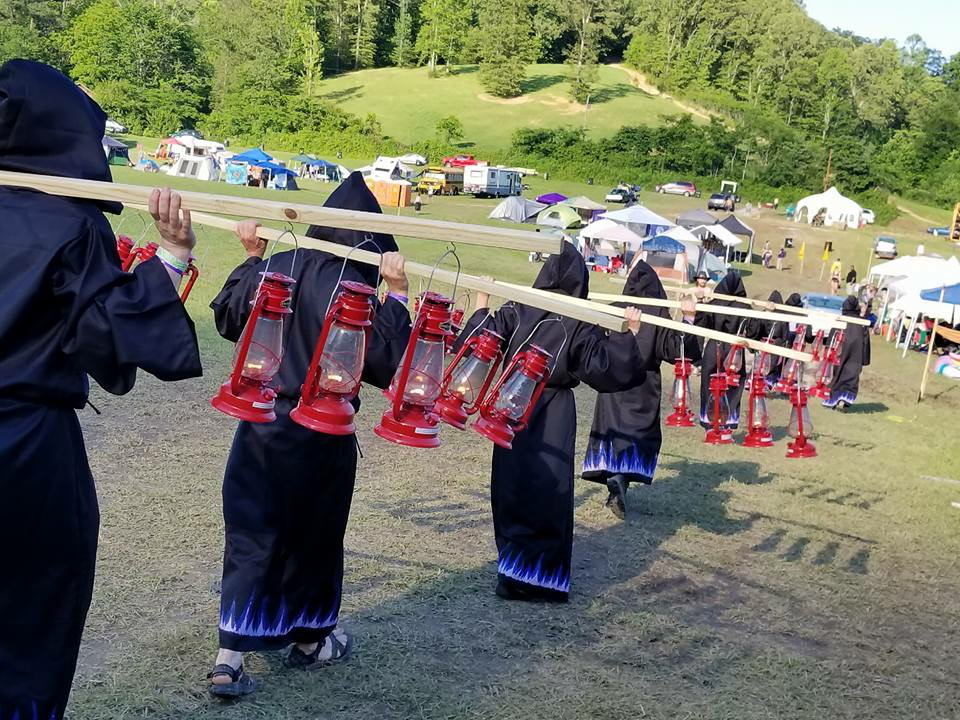
\includegraphics[width=\textwidth]{images/lamplighters.jpeg}
\caption{Lamplighters at work. Image courtesy of Johnny “Twaffle” Benton, 2017.}
\label{fig:lamplighters2017}
\end{figure}
